\documentclass[tikz,border=8pt]{standalone}
% Shared look for every TikZ diagram. Load with \input{../../tools/tikz-style.tex}
\usepackage[T1]{fontenc}
\usepackage{lmodern}
\renewcommand{\sfdefault}{lmr}  % diagrams use the same serif as the text
\usetikzlibrary{arrows.meta, positioning, shapes.geometric, calc, fit, backgrounds}
\definecolor{cblue}{HTML}{4C78A8}
\definecolor{corange}{HTML}{F58518}
\definecolor{cgreen}{HTML}{54A24B}
\definecolor{cred}{HTML}{E45756}
\definecolor{cpurple}{HTML}{B279A2}
\definecolor{cgrey}{HTML}{6B6B6B}
\tikzset{
  every picture/.style={font=\sffamily, line width=1.2pt},
  box/.style={draw=#1, fill=#1!12, rounded corners=4pt, align=center, inner sep=7pt, minimum height=1.1cm},
  box/.default=cgrey,
  arrow/.style={-{Stealth[length=3mm]}, draw=cgrey, line width=1.4pt},
  title/.style={font=\sffamily\bfseries\Large},
  note/.style={font=\sffamily\small, text=cgrey, align=center},
}
\AtBeginDocument{\hyphenpenalty=10000 \exhyphenpenalty=10000}

% Section 5.1 worked example: a = (1, 2), b = (4, 5), b - a = (3, 3), dot product 18, d = sqrt(18) = 4.24
\begin{document}
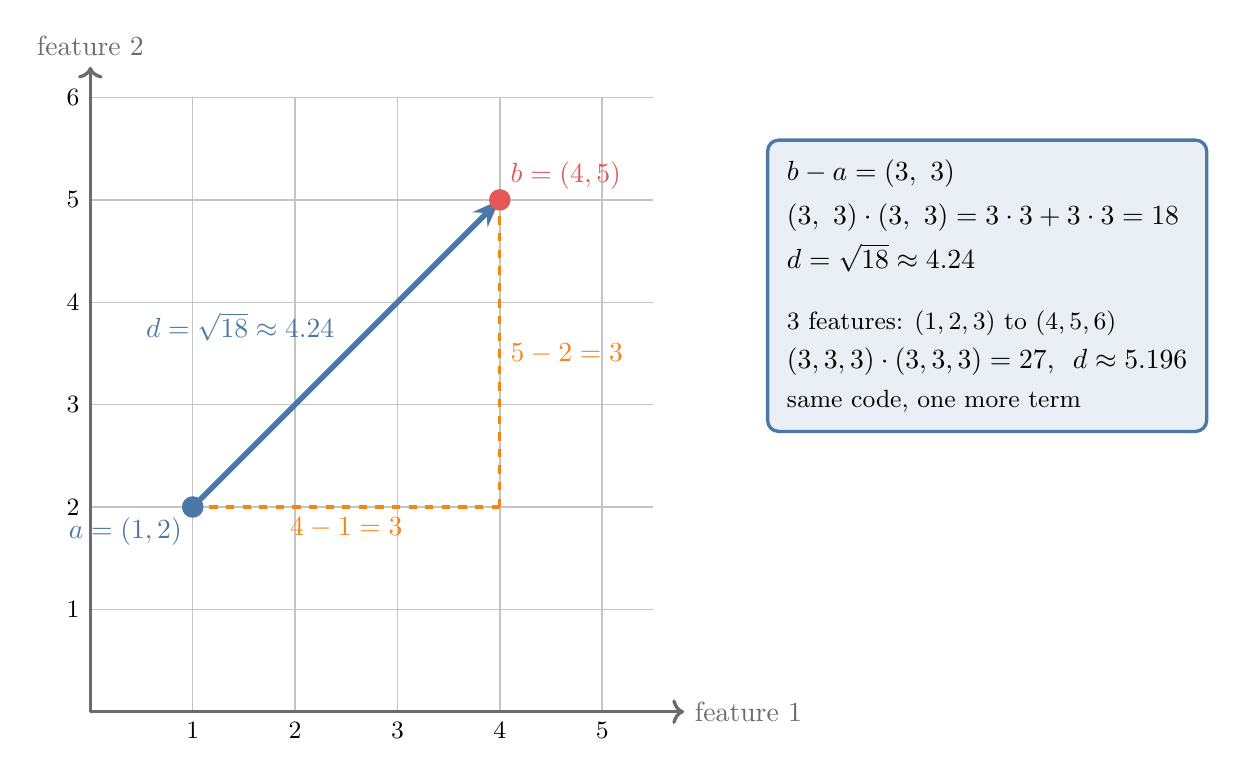
\begin{tikzpicture}[scale=1.3]
  \draw[cgrey!40, line width=0.5pt] (0,0) grid (5.5,6);
  \draw[->, cgrey] (0,0) -- (5.8,0) node[right] {feature 1};
  \draw[->, cgrey] (0,0) -- (0,6.3) node[above] {feature 2};
  \foreach \x in {1,...,5} \node[below, font=\small] at (\x,0) {\x};
  \foreach \y in {1,...,6} \node[left, font=\small] at (0,\y) {\y};
  \draw[corange, dashed] (1,2) -- node[below] {$4 - 1 = 3$} (4,2);
  \draw[corange, dashed] (4,2) -- node[right] {$5 - 2 = 3$} (4,5);
  \draw[-{Stealth[length=3.5mm]}, cblue, line width=2pt] (1,2) -- node[above left, text=cblue, align=center] {$d = \sqrt{18} \approx 4.24$} (4,5);
  \fill[cblue] (1,2) circle (3pt) node[below left] {$a = (1, 2)$};
  \fill[cred] (4,5) circle (3pt) node[above right] {$b = (4, 5)$};
  \node[box=cblue, anchor=north west, align=left, font=\normalsize] at (6.6,5.6) {%
    $b - a = (3,\ 3)$\\[4pt]
    $(3,\ 3)\cdot(3,\ 3) = 3\cdot 3 + 3\cdot 3 = 18$\\[4pt]
    $d = \sqrt{18} \approx 4.24$\\[10pt]
    {\small 3 features: $(1,2,3)$ to $(4,5,6)$}\\[2pt]
    $(3,3,3)\cdot(3,3,3) = 27$, \ $d \approx 5.196$\\[2pt]
    {\small same code, one more term}};
\end{tikzpicture}
\end{document}
